\documentclass{article}

\usepackage{tikz}
\usetikzlibrary{external}
\usetikzlibrary{decorations.pathmorphing}
\usetikzlibrary{decorations.markings}
\usetikzlibrary{shapes.arrows}
\usetikzlibrary{arrows}

\usetikzlibrary{positioning,fit,calc}
\usetikzlibrary{arrows.meta}
\usetikzlibrary{calc,fadings,decorations.pathreplacing}
%\usetikzlibrary{arrows.spaced}
\usetikzlibrary{decorations.pathmorphing}

\usepackage[compat=1.1.0]{tikz-feynman}

\usepackage{varwidth}
\usepackage{epstopdf}
\usepackage{amssymb}
\usepackage{relsize}

\tikzset{external/system call={lualatex
      \tikzexternalcheckshellescape -halt-on-error -interaction=batchmode
-jobname "\image" "\texsource"}}
%\tikzset{external/force remake}
\tikzexternalize % activate!

\begin{document}



\begin{figure}
\begin{center}
   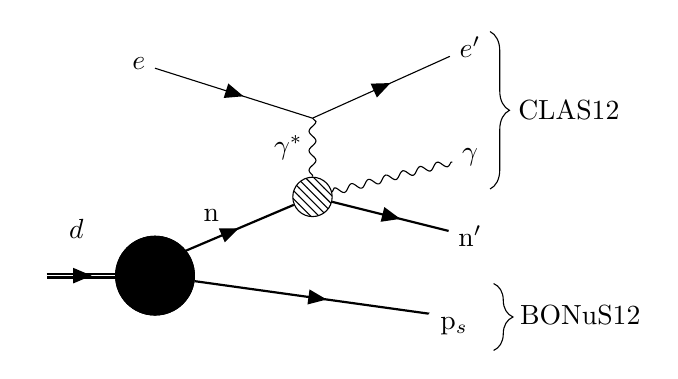
\begin{tikzpicture}[
         nucleon/.style = {thick,fermion},
         deuteron/.style = {double,thick,arrow size=0.5pt, 
         postaction={decorate}, decoration={markings, mark=at position 0.70 
         with {\arrow[scale=0.6]{triangle 45}}}}]

      \begin{feynman}
         \vertex                                            (n0) {};
         \vertex[large, blob, fill=black,right=1.5cm of n0] (n1) {};

         \vertex[above right=0.6cm and 0.5 of n0]   (Ain) {$d$};

         % incoming A nucleons
         \vertex[above = 0.15cm of n0]  (n01){~};
         \vertex[above = 0.30cm of n0]  (n02){~};
         \vertex[above = 0.45cm of n0]  (n03){~};
         \vertex[below = 0.15cm of n0]  (n04){~};
         \vertex[below = 0.30cm of n0]  (n05){~};
         \vertex[below = 0.45cm of n0]  (n06){~};

         \vertex[above = 0.15cm of n1]  (n11){~};
         \vertex[above = 0.30cm of n1]  (n12){~};
         \vertex[above = 0.45cm of n1]  (n13){~};
         \vertex[below = 0.15cm of n1]  (n14){~};
         \vertex[below = 0.30cm of n1]  (n15){~};
         \vertex[below = 0.45cm of n1]  (n16){~};

         %\vertex[label={[label distance=0.2cm]-130:label},blob, fill=black, 


         \vertex[below right=0.2cm and 2.5cm of n1]   (n2)  ;
         \vertex[below right=0.2cm and 2.55cm of n11]  (n21) ;
         \vertex[below right=0.2cm and 2.45cm of n14]  (n24) ;

         \vertex[below right=0.3cm and 1.1cm of n2]   (n3)  ;
         \vertex[below right=0.8cm and 1.1cm of n21]  (n31) ;
         \vertex[below right=0.8cm and 1.1cm of n24]  (n34) ;


         %dvcs vertex
         \vertex[small, blob, above right=1.0cm and 2.0cm of n1] (a0) {};


         % e,e'gamma vertex 
         \vertex[above=1.0cm of a0]                  (q0);
         \vertex[below right=0.5cm and 2.0cm of a0]  (a1) {n$^{\prime}$};
         \vertex[above=1.0cm of a1]                  (q1){\(\gamma\)};

         % fsi
         \vertex[above right=0.1cm and 2.7cm of n1] (fsi);
         \vertex[left=1.15cm of a1]              (a10);

         % electron
         \vertex[above left=0.5cm and 2.0cm of q0]  (e0) {\(e\)};
         \vertex[above=1.4 of q1]   (e1) {\(e^{\prime}\)};

         \diagram*{
            (e0) -- [fermion] (q0) -- [fermion] (e1),
            (n11) -- [nucleon, edge label = n] (a0),
            (a0)  -- [nucleon] (a1),
            (a0) -- [photon, edge label = \(\gamma^{*}\)] (q0),
            (q1) -- [photon] (a0),
            (n0) -- [deuteron](n1) -- [nucleon](n3),
         };

         %fill in the blob again
         \vertex[large, blob, fill=black,right=1.5cm of n0] {};

         % bonus12 detection
         \draw [decoration={brace,amplitude=7pt}, decorate]
          ($(n3.east)+(0.7cm,0.4cm)$) -- ++(-0.0cm,-0.85cm);
          \node[] at ($(n3.east)+(1.8cm,-0.0cm)$) {BONuS12};

         % CLAS12 detection
         \draw [decoration={brace,amplitude=7pt}, decorate] 
         ($(e1.east)+(0.0cm,0.2cm)$) -- ++(-0.0cm,-2.0cm);
         \node[] at ($(e1.east)+(1.0cm,-0.8cm)$) {CLAS12};

         \draw[fill,white,rotate=-35] ($(n3)-(0.10cm,0.3cm)$) rectangle 
         ($(n3)+(0.10cm,0.3cm)$);
         \vertex[below right=-0.1cm and -0.1cm of n3]    (pminus1) {p$_{s}$};

      \end{feynman}
   \end{tikzpicture}
\end{center}
\caption{Incoherent DVCS on D}
\end{figure}





\begin{figure}
\begin{center}
   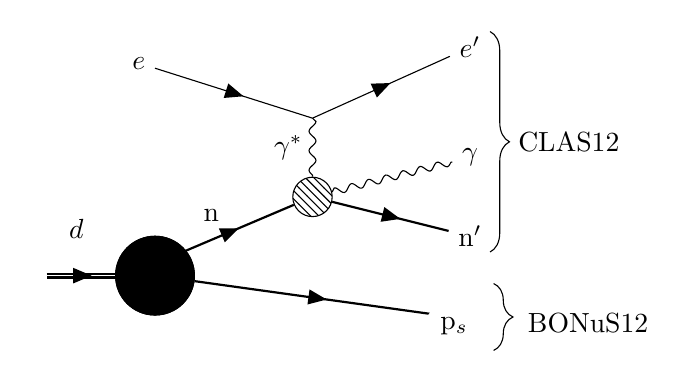
\begin{tikzpicture}[
         nucleon/.style = {thick,fermion},
         deuteron/.style = {double,thick,arrow size=0.5pt, 
         postaction={decorate}, decoration={markings, mark=at position 0.70 
         with {\arrow[scale=0.6]{triangle 45}}}}]

      \begin{feynman}
         \vertex                                            (n0) {};
         \vertex[large, blob, fill=black,right=1.5cm of n0] (n1) {};

         \vertex[above right=0.6cm and 0.5 of n0]   (Ain) {$d$};

         % incoming A nucleons
         \vertex[above = 0.15cm of n0]  (n01){~};
         \vertex[above = 0.30cm of n0]  (n02){~};
         \vertex[above = 0.45cm of n0]  (n03){~};
         \vertex[below = 0.15cm of n0]  (n04){~};
         \vertex[below = 0.30cm of n0]  (n05){~};
         \vertex[below = 0.45cm of n0]  (n06){~};

         \vertex[above = 0.15cm of n1]  (n11){~};
         \vertex[above = 0.30cm of n1]  (n12){~};
         \vertex[above = 0.45cm of n1]  (n13){~};
         \vertex[below = 0.15cm of n1]  (n14){~};
         \vertex[below = 0.30cm of n1]  (n15){~};
         \vertex[below = 0.45cm of n1]  (n16){~};

         %\vertex[label={[label distance=0.2cm]-130:label},blob, fill=black, 


         \vertex[below right=0.2cm and 2.5cm of n1]   (n2)  ;
         \vertex[below right=0.2cm and 2.55cm of n11]  (n21) ;
         \vertex[below right=0.2cm and 2.45cm of n14]  (n24) ;

         \vertex[below right=0.3cm and 1.1cm of n2]   (n3)  ;
         \vertex[below right=0.8cm and 1.1cm of n21]  (n31) ;
         \vertex[below right=0.8cm and 1.1cm of n24]  (n34) ;


         %dvcs vertex
         \vertex[small, blob, above right=1.0cm and 2.0cm of n1] (a0) {};


         % e,e'gamma vertex 
         \vertex[above=1.0cm of a0]                  (q0);
         \vertex[below right=0.5cm and 2.0cm of a0]  (a1) {n$^{\prime}$};
         \vertex[above=1.0cm of a1]                  (q1){\(\gamma\)};

         % fsi
         \vertex[above right=0.1cm and 2.7cm of n1] (fsi);
         \vertex[left=1.15cm of a1]              (a10);

         % electron
         \vertex[above left=0.5cm and 2.0cm of q0]  (e0) {\(e\)};
         \vertex[above=1.4 of q1]   (e1) {\(e^{\prime}\)};

         \diagram*{
            (e0) -- [fermion] (q0) -- [fermion] (e1),
            (n11) -- [nucleon, edge label = n] (a0),
            (a0)  -- [nucleon] (a1),
            (a0) -- [photon, edge label = \(\gamma^{*}\)] (q0),
            (q1) -- [photon] (a0),
            (n0) -- [deuteron](n1) -- [nucleon](n3),
         };

         %fill in the blob again
         \vertex[large, blob, fill=black,right=1.5cm of n0] {};

         % bonus12 detection
         \draw [decoration={brace,amplitude=7pt}, decorate]
          ($(n3.east)+(0.7cm,0.4cm)$) -- ++(-0.0cm,-0.85cm);
          \node[] at ($(n3.east)+(1.9cm,-0.1cm)$) {BONuS12};

         % CLAS12 detection
         \draw [decoration={brace,amplitude=7pt}, decorate] 
         ($(e1.east)+(0.0cm,0.2cm)$) -- ++(-0.0cm,-2.8cm);
         \node[] at ($(e1.east)+(1.0cm,-1.2cm)$) {CLAS12};

         \draw[fill,white,rotate=-35] ($(n3)-(0.10cm,0.3cm)$) rectangle 
         ($(n3)+(0.10cm,0.3cm)$);
         \vertex[below right=-0.1cm and -0.1cm of n3]    (pminus1) {p$_{s}$};

      \end{feynman}
   \end{tikzpicture}
\end{center}
\caption{Incoherent DVCS on D}
\end{figure}

\end{document}



